% \hyperref[sec:sec7]{\section{為什麼立法會一天到晚都在拉布而不議事?}}
\section{為什麼立法會一天到晚都在拉布而不議事?}
\label{sec:sec23}

由於立法會有先天的議會和選舉制度缺陷,所以即使沒有拉布,本來就不能有效議事。在一個正常的議會中,議員和議案的質素最終會通過民意反映到議席之上,做得不好就要下台。同樣的制衡難以在香港的立法會發生,建制派幾近永遠是議會的多數派,議會議事也就變得行禮如儀了。因此,雖然拉布在公眾眼中好像把立法會變得不能議事,但考慮到在議會議事的目的本來就是要促進和反映公眾辯論,而拉布可以吸引到公眾對某些議題的關注,則可說拉布和議事並不矛盾,而是繞了個彎達到議會本來應有的功能,為真正的議事帶來契機。

所謂拉布或冗長辯論,是指少數議員在明知不能阻擋某個議案獲投票通過,便利用各種方式來拖延議會程序,一方面引發公眾關注,另一方面增加通過此議案的時間成本。畢竟議會會期有限,如果拉布策略成功,得到市民支持,或可迫使對方撤回議案,甚至迫使議案因為會期結束而失效。

拉布在世界各地的不少議會均有範例,美國國會參議院就有 filibuster 的傳統,台灣則很有創意地把此詞譯成「廢力把事拖」。美國參議院的議事規則規定參議員可就任何題目發言而時間不限,有參議員就曾經連續二十四小時發言,也有參議員朗讀聖經章節和兒童故事,甚至把電話簿和食譜從頭到尾諗一遍。日本參議院則有所謂「牛步戰術」,即在投票時採用極為緩慢的步伐走向投票箱,平常數十秒的步程變成數分鐘,如果所反對派的議員都加入便可拖上半天。

在香港的立法會,建制陣營基於畸型選舉制度的幫助而幾近可護送任何議案通過,拉布便成為了非建制陣營少數可用的反抗手段。不過,特區成立以來的首次立法會拉布,卻是來自建制陣營。一九九九年審議廢除市政局和區域市政局的時候,表決前剛好有建制陣營的議員未能趕及回到會議廳,政府為免議案被否決便利用了議事規則中政府總結發言時間不限的規定,不停拖長官員發言直到有足夠建制陣營的議員趕及回到會議廳為止。

要在議會拖延時間的方法有很多。以二零零九年十二月至二零十零年一月的高鐵撥款審議為例,非建制陣營的議員就透過不斷向官員提問使得表決日期被一再壓後。不過這次經驗嚴格來說不算拉布,因為高鐵作為特區成立以來最大規模的基建工程,議員當時所問的問題都有實質意義。而由於議會拉布文化尚未成型,議員們都避諱以過於鎖碎的辯論來拖延時間。

到了二零一二年的《立法會議席出缺安排議案》,政府提出限制議員辭職後再次參選,引發黃毓民等非建制陣營議員發動拉布抗爭。首先,他們就議案提出了合共1307條的修訂。這些修訂的內容十分廣泛,例如規定如有議員「因未獲正式審訊,被古巴政府囚禁超過一個月,又同日辭職,一個月內其中一人獲釋放,條例就不適用」,然後把國家名字改為朝鮮、中國、津巴布韋和越南等,衍生出多項修訂。然後他們在審議階段輪流就這些修訂發言,例如介紹古巴的政治局勢,以求一方面拖延時間,同時避免被主席裁定離題或重複內容。又有另一組的修訂為「若議員因為患上肝癌辭職,一個月內被確定無患肝癌,條例就不適用」,然後再換上另外十六組不同疾病,衍生出十七項修訂。有議員討論到相關修訂時,更詳細分享「露德聖水」傳聞神蹟,以說明患病又突然康復的可能。有些修訂則針對個別字眼,引發「實行」和「施行」的用字分別討論。

由於這些修訂大多十分鎖碎,建制陣營的議員在審議時難以集中精神,有些議員在坐位練習書法,或者閉目養神。但他們這樣做卻又會給予機會非建制陣營的議員提出質疑,例如梁國雄議員就曾經向會議主席報告黃定光議員睡著了,擔心他有生命危險,引起的議論又成為另一種拖延時間的方法。

不過最有效的拖延戰術則是人數點算。立法會內不同會議都有法定人數的限制,建制陣營的議員由於不少都是企業高層,未必能時刻會在立法會大樓出現。而就算身處大樓,也可能因為要會見市民或團體代表而未能時刻坐在會議廳開會。因此,只要非建制陣營的議員集體離場,只留下少數代表負責拖延審議,會議廳便很容易因為法定人數不足而流會。按當時的議事規則,立法會大會的會期逢星期三開始起算,萬一流會的話不輪是在星期三、四或五發生,都要留待下一個星期三才能繼續,可以拖延很多時間。

而就算未能成功促使流會,由於每次點算人數最多可以花十五分鐘的鳴鐘時間來等待議員回到議事廳,僅僅是這程序本身已可花掉不少時間。在二零一五至一六年度的立法會大會,就累計點人數共556次,耗用時間107小時56分鐘。

這些拉布手段把立法會的時間都消耗在執行程序之上,無形中就拿走了本來可以用來審議其他議案的時間。視乎不同的政治觀點,這可以是好事也可以是壞事。例如大埔區議會本來建議動用五千萬於林村建設旅遊設施,被批評為「林村天安門」,當地居民不少都認為交通不能負荷更多遊客而反對計劃。撥款建議因為拉布而未能於二零一六年立法會會期完結時獲得通過,及後大埔區議會決定撤回建議,改為建議把撥款用於藝術和醫療。在這件事情上,拉布就幫助了少數議員成功阻擋議會強行通過議案。

反過來說,反對拉布的議員則會指責拉布的議員阻礙議會運作,使得一些市民支持的項目(如興建學校或醫院等的撥款申請)也因為拉布而無法審議。不過,政府其實有權調動議案的審議程序,讓立法會先處理爭議較少的議案。所以準確來說,拉布其實無論對政府和建制陣營或是非建制陣營來說都是一種政治博奕的手段,兩邊都要時刻計算市民會把否接受議會癱瘓,和會把責任放在誰的身上。

按香港中文大學的民意調查顯示,有超過五成受訪者原則上不支持議員就具爭議性的議題拉布,支持的只有一成多。綜合上文提及的立法會碎片化的現象,非建制陣營在拉布議題上處於十分不利的位置。他們既有少數支持者希望他們多利用拉布手段拖垮具爭議性的議題,卻同時有另一批支持者不同意這種手法。在比例代表制的選舉制度下,便衍生出非建制陣營的各個成員自顧選擇走不同的抗爭路線,但卻在公眾眼中加深了非建制陣營未能團結的印象。

\begin{figure}[htbp]
    \centering
    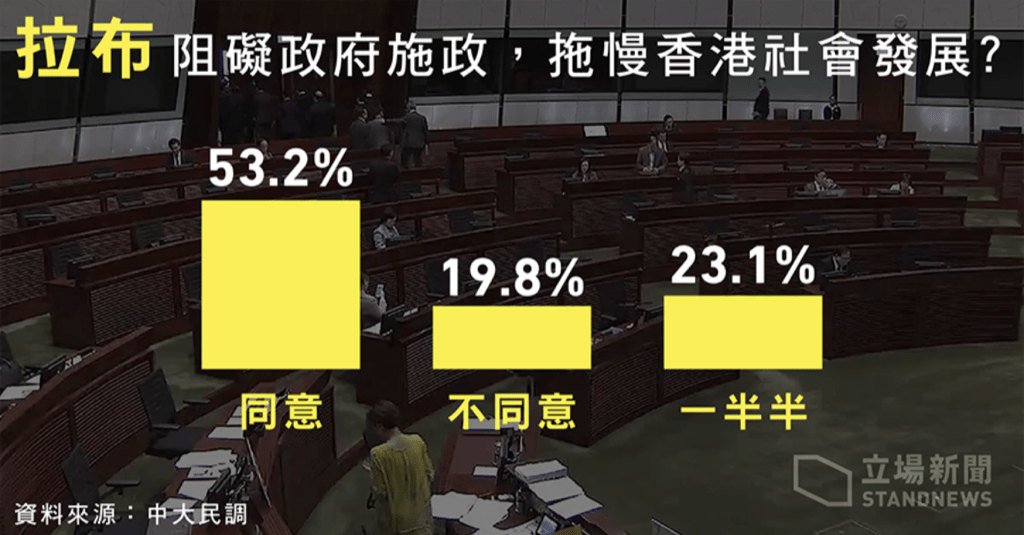
\includegraphics[width=0.7\textwidth]{c23/h-klesson1-038.png}
    \caption{民調顯示市民對拉布並不支持} 
\end{figure}

對於建制陣營來說,他們一方面不喜歡坐在會議廳聆聽冗長辯論,也見到非建制陣營在拉布議題上所處的尷尬位置,固然不會放過以此攻擊對手,把拉布描繪為一件不利民生的事情。由於一般市民未必理解或認同拉布作為回應立法會制度缺陷的手段,加上非建制陣營本身的碎片化,要回應攻擊也十分困難。到了二零一七年年底,由於有非建制陣營的議員被取消資格(見\hyperref[sec:sec22]{問題二十二}),立法會首次出現無論是功能界別或是地區直選都由建制陣營佔過半數的情況,由建制陣營議員提出的議案不再受「分組點票」所限以不能通過。於是乎,他們便趁機修改了議事規則,大幅度減少各種拖延立法會程序的機會。

相對於很多外國的議會,香港立法會對拉布本來沒有很清晰的規範。回到美國國會參議院的冗長辯論,就有所謂的終結發言議案,即如果獲參議院五分之三議員的同意,可終止發言程序把議案付諸表決。香港立法會沒有這樣的規定,過去各拉布戰的結束都是由會議主席一個人裁決終止,從議會管治來說並不理想。加上立法會的制度缺陷使得主席幾乎必然是由建制陣營議員擔任,由主席一人作出終止發言程序的裁決則更難服眾。

如果香港的立法會已達至全面普選,則近年的拉布風潮或可被理解為濫用程序,通過修改議事規則來處理也算合理。例如香港可考慮採用類似美國參議院的方式處理拉布問題,應可平衝少數意見的同時又不會讓議會被極少數拖垮。不過建制陣營的議事規則修訂,卻是把更多的權力交給會議主席,例如處理修正案和流會後何時復會。當時就有多名學者發起了聯署聲明,批評此舉「嚴重削弱立法會現時僅有些微監察政府的權力」。

\begin{figure}[htbp]
    \centering
    
\includegraphics[width=0.7\textwidth]{c23/h-klesson1-039.png}
    \caption{學界不支持修改議事規則(學術自由學者聯盟圖片)}
\end{figure}

相對來說,雖然美國也常有意見認為要削減冗長辯論,但無論誰是多數黨都不敢貿然推行,因為他們明白自己今天是多數黨,下屆卻可以變成少數黨,打壓少數的做法有朝一日會害及自己。但在香港,建制陣營很有信心自己永遠都是立法會的多數,所以不擔心通過修訂後自己日後會因而有所損失。

香港立法會的拉布問題並非單純出於個別議員濫用程序,而是立法會本身無法代表民意和制度上無法履行正常的議事職能。有個別議員採取在議事廳內各種方式抗爭,無論是口頭甚至行動上的衝突,又或用各種方式拖延程序,背後都指向立法會本身在相當部分的市民心目中欠缺認授,所以這些議員的行動才能得到支持。而即使這些議事廳內的抗爭方式被終止,只要背後的認授問題沒有解決,則問題仍會如擠氣球一樣,從議事廳內轉移到議事廳外,甚至而更高社會成本的方式爆發。

\rule[-10pt]{15cm}{0.05em}

伸延閱讀:

Cullen R, 2018, Filibustering: Flawed in Principle and Bad for Hong Kong, \textit{IPP Review Mar. 09, 2018}.

Kaeding MP (2017) The Rise of “Localism” in Hong Kong, \textit{Journal of Democracy 28:1}, p157-171.


網上資源:

\href{https://thestandnews.com/politics/中大民調-逾半市民不支持拉布/}{立場報道(2017)中大民調:逾半市民不支持拉布 近半贊成改議規:立場新聞,2017年12月5日}

\href{https://thestandnews.com/politics/學者反議規修訂-逾4000人網上聯署/}{立場報道(2017)學者反議規修訂 逾4000人網上聯署:立場新聞,2017年12月13日}